\pagelayout{wide} % No margins
\addpart{Capítulo 2: Patrones creacionales}
\pagelayout{margin} % Restore margins


\setchapterpreamble[u]{\margintoc}
\chapter{Patrones Creacionales}
\labch{cap3}

\section{{¿Qué son los patrones creacionales?}}

Los patrones de diseño creacionales se centran en abstraer el proceso de creación e instanciación de los objetos con el propósito permitir al sistema ser independiente a la forma en la cual los objetos o estructuras de objetos complejos son creados y representados en el dominio de nuestra aplicación. Generalmente, los patrones creacionales son utilizados con el objetivo de separar la lógica encargada de la creación de objetos y encapsularla para ser reutilizada de manera transversal.

Estos patrones se rigen bajo dos ideas principales que hacen posible su reutilización independiente de la tecnología, enfoque o lenguaje de programación orientado a objetos: (i) encapsular el conocimiento y la lógica detrás de la creación de objetos y (ii) ocultar el mecanismo utilizado para su instanciación. Gracias a ello, los patrones creacionales permiten que la implementación sea transparente para el desarrollador, ofreciendo las herramientas necesarias para definir como, cuando, por qué y para qué se crea un objeto o una estructura de datos compleja, lo cual garantiza que las soluciones sean altamente flexibles.

\section{¿Por qué debería usar patrones creacionales?}

Durante el proceso de desarrollo de proyectos de software, nos encontramos de manera frecuente con que cada desarrollador aplica su propia lógica al momento de realizar una implementación, lo cual es entendible ya que cada persona es un mundo y tiene la capacidad de resolver un problema de muchas maneras diferentes. Sin embargo, cuando nos enfrentamos a dominios específicos nos damos cuenta que muchas veces el desarrollo de software se encuentra con problemas comunes y recurrentes que pueden ser abstraidos y agrupados en estructuras transversales que puedan ser reutilizadas por otros. Sunpongamos que nuestra aplicación requiere crear una instancia unica e inmutable que pueda ser accedida de manera global, o necesitamos crear/clonar un objeto complejo sin preocuparnos por su estructura interna; en estos casos y en muchos otros, los patrones creacionales nos ofrecen la herramientas necesarias para crear e instanciar objetos de manera transparente y reutilizable sin preocuparnos por la lógica interna de los objetos y clases involucrados.

En general, algunos de los escenarios mas comunes en los que es recomendable utilizar los patrones creacionales son:

\begin{itemize}
	\item Al sistema no le interesa conocer la forma en la cual se crean los objetos que va a utilizar.
	\item Es necesario crear diferentes representaciones de un objeto complejo.
	\item Se requiere realizar la instanciación de estructuras de datos complejas en tiempo de ejecución
	\item El sistema solo necesita una instancia que pueda ser accedida de manera global por toda la aplicación
	\item La instanciación de nuevos objetos debe ser flexible sin modificar las estructuras existentes.
\end{itemize}

\section{Patrones existentes}

A continuación, se presentarán de manera ordenada cada uno de los patrones creacionales de acuerdo a su definición, motivación, como lograr la definición del patrón, las situaciones en las cuales se recomienda su aplicación, diseño en UML, un ejemplo conceptual (no necesariamente relacionado a un problema informático) y su implementación práctica paso a paso con el objetivo de comprender el patrón a un mayor nivel de detalle.

\subsection{Singleton}

\textbf{Definición:} El patron singleton o de instancia única tiene el objetivo de restringir la creación de una clase a una sola instancia que pueda ser accedida de manera global. Este parón es quizás el mas sencillo debido a que no presenta un alto grado de complejidad y no requiere técnicas elaboradas de desarollo para llevar a cabo su implementación.

\textbf{Motivación:} En ocasiones necesitamos que una clase tenga exactamente una instancia, como por ejemplo para la definición de una instancia única base de datos, una variable de acceso global a una estructura de datos compleja o cuando nuestra aplicación realiza procesamiento de datos concurrentes que requieren acceder a un objeto de instancia común.

\textbf{¿Como puedo implementar un singleton?:} Para crear un singleton, deberíamos ser capaces de definir la estrutura necesaria para asegurar que un objeto de una clase cualquiera solo pueda ser instanciada una vez, una de las formas mas comunes de hacerlo es mediante un constructor privado que impida a clases externas realizar su instanciación y ocultar la lógica encargada de la instanciación del objeto dentro de un método público definido en la clase.

\textbf{Escenarios de aplicación:}

\begin{itemize}
	\item Debe existir exactamente una instancia de una clase y su acceso debe ser global
\end{itemize}

\textbf{Modelo UML:}

El aspecto mas importante de este patrón es la definición de un método privado que se encargue de la instanciación del objeto, lo cual garantiza que el objeto solo pueda ser creado una vez, así cuando un Cliente específico requiera utilizar el objeto solo deba preocuparse por obtener la instancia.

\begin{figure}[H]
	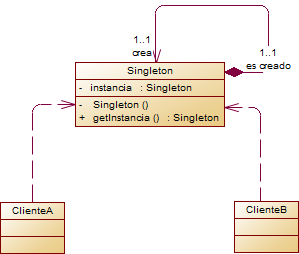
\includegraphics[width=0.7\textwidth]{images/creational/singleton/singleton.png}
\end{figure}

\textbf{Ejemplo conceptual:} De acuerdo a las teorías actuales aceptadas en cosmología, existe un unico Universo en el cual vivimos y existe todo lo que conocemos. Imaginemos el mecanismo que pudo llevarse a cabo para permitir que este Universo existiera, hasta donde sabemos solo existe una instancia de nuestro Universo y no hay pruebas concluyentes que indiquen la existencia de otros Universos. Por algún motivo fuera de nuestro entendimiento la naturaleza decidió que el Universo fuera un singleton. A continuación intentaremos abstraer la lógica necesaria para crear un Universo y plasmarlo en un programa computacional.

Inicialmente, se podría pensar en la creación de una clase \textbf{SingletonUniverso} que se encargue de implementar la lógica necesaria para crear y mantener una sola instancia del Universo durante toda la ejecución del programa. Para ello, se define un constructor privado \textbf{SingletonUniverso()} que impida a otros crear nuevas instancias.

\begin{figure}[H]
	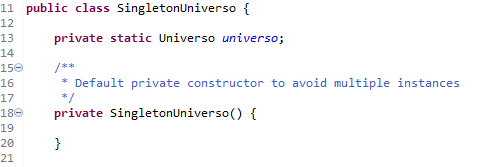
\includegraphics{images/creational/singleton/singletonExample1.png}
\end{figure}

Ya tenemos nuestro posible nuevo Universo, ahora es necesario implementar el mecanismo para que su instanciación sea única, el patrón singleton propone la creación de una función pública  \textbf{getInstancia()} que tendra cumplirá dos funciones: (i) crear una nueva instancia si no existe y (ii) retornar la instancia cuando esta ya exista. De manera opcional se pueden crear métodos adicionales que se encarguen de funciones específicas relacionadas al dominio de la aplicación.

\begin{figure}[H]
	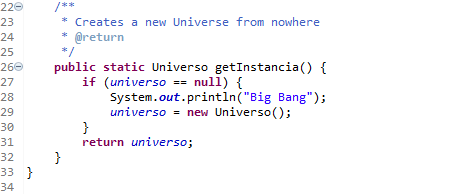
\includegraphics{images/creational/singleton/singletonExample2.png}
\end{figure}

Como se puede observar, la implementación del singleton no conlleva lógica adicional, una vez creada la definición general de la clase solo basta con que una clase externa requiera instanciar un Universo. De acuerdo a la forma en la cual fue definida la clase es imposible realizar su instanciación de manera directa, resultando en un error de compilación indicando que el constructor de la clase no es visible.

\begin{figure}[H]
	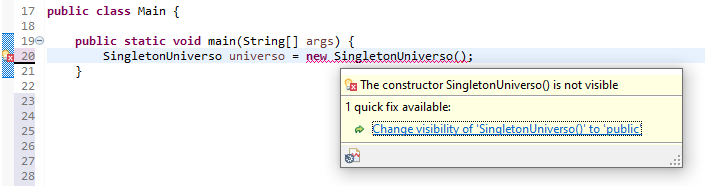
\includegraphics{images/creational/singleton/singletonExample3.png}
\end{figure}

Por otro lado, el patron garantiza que solo exista un Universo en nuestra aplicación, un usuario todopoderoso que requiera crear un nuevo Universo está obligado a invocar el método \textbf{getInstancia()}, si por alguna razón necesita crear uno nuevo se encontrará con que es imposible gracias a que el diseño solo permite una única instancia.

\begin{figure}[H]
	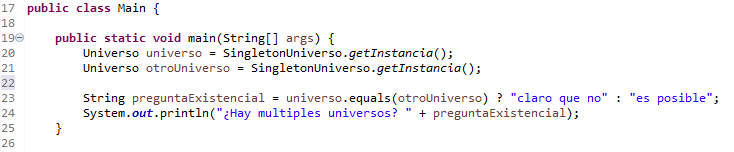
\includegraphics{images/creational/singleton/singletonExample4.png}
\end{figure}

Gracias a la flexibilidad ofrecida por los lenguajes orientados a objetos es posible identificar si dos instancias de una clase hacen referencia al mismo objeto, en particular, JAVA permite realizar una comparación con el método equals (que para este propósito es mas que suficiente), obteniendo que los dos Universos creados son en efecto el mismo, cumpliendo con el objetivo del patrón.

\begin{figure}[H]
	
\includegraphics{images/creational/singleton/singletonExample5.png}
\end{figure}

Un aspecto interesante del patrón singleton es que puede ser violado. Algunos lenguajes de programación como JAVA o C++ cuentan con librerías externas que permiten clonar una clase, acceder a las propiedades de clase a través de reflexión o deserializar de la clase, este tipo de operaciones permiten instanciar nuevos objetos saltando el control establecido por el singleton, lo cual viola el principio de unica instancia propuesta por el patrón. Existen diferentes técnicas que permiten evitar este comportamiento, por ejemplo lanzando una excepción en tiempo de ejecución que impida al usuario clonar el objeto o sobreescribir el método clone() para modificar su comportamiento.

Imaginemos un escenario en el cual un programador audaz decida de manera deliberada intentar clonar nuestro Universo implementando la interfaz \textbf{Cloneable}

\begin{figure}[H]
	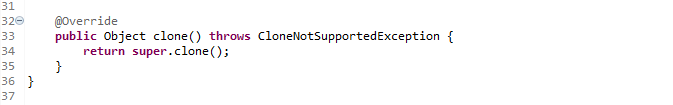
\includegraphics{images/creational/singleton/singletonExample6.png}
\end{figure}

Como resultado, nuestro amigo todopoderoso podría romper la regla de instancia única y crear múltiples Universos identicos al nuestro.

\begin{figure}[H]
	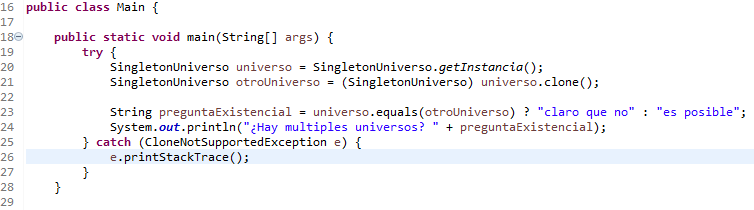
\includegraphics{images/creational/singleton/singletonExample7.png}
\end{figure}

Finalmente, el propósito del patrón se pierde

\begin{figure}[H]
	
\includegraphics{images/creational/singleton/singletonExample8.png}
\end{figure}

 Realizar este tipo de acciones no tiene sentido ya que destruyen el propósito del patrón. Por otro lado, es posible observar que la implementación comienza a volverse engorrosa porque obliga al desarrollador a validar escenarios adicionales de excepción, lo que limita el alcance de la solución y la vuelve menos flexible.

De manera análoga al caso anterior, el patrón podría ser violado mediante reflexión de clases u otros artilugios ingeniosos, sin embargo se debe tener presente que este no es el objetivo del patrón. Para evitar estos escenarios no deseados el desarrollador puede decidir agregar implementaciones adicionales al singleton que dote a la clase con los mecanismos necesarios para evitar estos comportamientos. Uno de los aspectos mas destacables en los esfuerzos por evitar esta situaciones se centra en realizar mejoras a los lenguajes de programación para evitar que se puedan realizar estas acciones, por ejemplo, a partir de la versión de Java 8 ya no es posible instanciar un singleton utlizando reflexión. Otros autores proponen apoyarse en el uso de estructuras como los Enumerados (o Enum) que limitan la creación de objetos. De acuerdo a Joshua Bloch en su libro "Java Best Practices", el uso de enumeradores permite facilitar la implementación de un Singleton y facilitar el trabajo de pruebas unitarias asociadas a la clase. Finalmente se debe tener siempre en cuenta que la decisión final de respetar la arquitectura es del desarrollador.
\subsection{Prototype}

\textbf{Definición:} El patron prototype o prototipo tiene la finalidad de clonar nuevos objetos a partir de una instancia de objeto creada a priori. Para ello, el prototipo toma como base una estructura definida y realiza su clonación.

Un aspecto bastante importante que se debe tener en cuenta cuando se habla de clonación de objetos es que existen dos opciones al momento de clonar un objeto:

\begin{itemize}
	\item \textbf{Clonación superficial:} El proceso de instanciación se limita a crear una copia de los atributos de tipo primitivo (int, long, char, boolean, etc), por otro lado, los tipos de dato complejos son referenciados en la copia. Por lo tanto, si se realiza una modificación de un tipo de dato complejo en la copia, este afectará de manera directa al objeto original
	\item \textbf{Clonación profunda:} Se realiza una copia campo a campo del objeto original, resultando en que la copia es una instancia diferente miembro a miembro. Esto implica un costo de procesamiento mayor debido a que el sistema debe crear la estructura completa del objeto original. Sin embargo, modificar la copia no tendría ninguna consecuencia en el objeto original.
\end{itemize}


\textbf{Motivación:} En muchas ocasiones el costo de crear un nuevo objeto desde cero puede ser muy alto, en estas situaciones es adecuado clonar una estructura existente que actue como un prototipo y modifiar aquellos atributos que sean necesarios. Por otro lado, es posible que un usuario requiera crear una instancia identica de un objeto existente y no esté interesado en la manera en la cual se creó el objeto original. El patrón prototipo tiene la ventaja de ocultar la complejidad asociada a la creación de nuevas instancias.

\textbf{¿Como puedo implementar un prototype?:} El patrón prototipo delega la responsabilidad de clonar el objeto al objeto original a través de una interfaz común que se puede encargar de crear la copia del objeto. Generalmente, lenguajes orientados a objetos como JAVA permiten realizar la clonación mediante la implementación de la interfaz Cloneable que se encarga de realizar todo el proceso de copiar todos los atributos a una nueva instancia.

\textbf{Escenarios de aplicación:}

\begin{itemize}
	\item Es necesario crear nuevas instancias de una clase compleja que cumplen con la misma estructura de un modelo base.
	\item Se requiere instanciar objetos con una estructura común
	\item Se requiere crear objetos idénticos en tiempo de ejecución.
	\item La aplicación necesita crear multiples objetos con las mismas características evitando un consumo excesivo de recursos.
\end{itemize}

\textbf{Modelo UML:}

El corazón del patrón se centra en la definición de una interfáz encargada de permitir que la clonación del objeto sea transparente para el cliente, a partir de esto es posible crear las implementaciones necesarias de acuerdo a las necesidades del desarrollo.

\begin{figure}[H]
	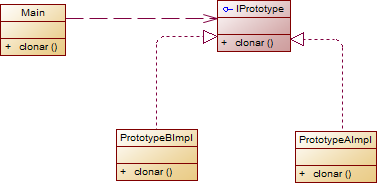
\includegraphics[width=0.9\textwidth]{images/creational/prototipe/prototype.png}
\end{figure}

\textbf{Ejemplo conceptual:} Científicos del instituto Roslin en Edimburgo lograron clonar el primer mamífero con éxito. Para ello se basaron en las células de una oveja finlandesa y tomaron su base genética como prototipo para obtener una oveja idéntica llamada Dolly. En este momento, se requiere realizar un programa computacional que emule este proceso a través de un proceso de clonación que permita al usuario clonar ovejas y conocer sus características individuales.

De acuerdo a las condiciones presentadas durante el experimento, existe una oveja que actua como prototipo a ser clonado, esto se puede lograr mediante la creación de una interfaz encargada de crear una copia exacta del objeto. Para ello, JAVA dispone de la interfaz Cloneable que permite realizar este proceso de manera transparente al usuario.

\begin{figure}[H]
	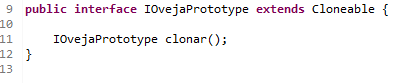
\includegraphics{images/creational/prototipe/prorotypeExample1.png}
\end{figure}

Tomando la interfaz como base, es posible crear nuevas ovejas mediante implementaciones específicas que ocupen el método clonar.

\begin{figure}[H]
	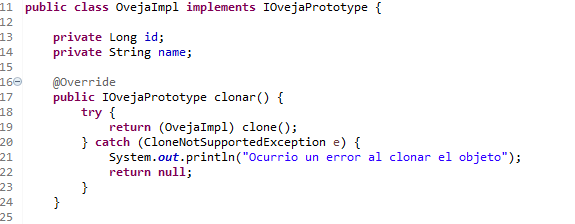
\includegraphics{images/creational/prototipe/prorotypeExample2.png}
\end{figure}

Adicionalmente, se sobreescribe el método toString() para presentar al usuario las propiedades básicas de la oveja.

\begin{figure}[H]
	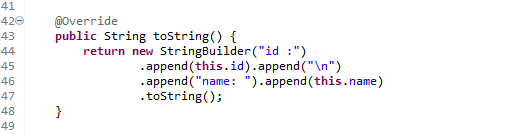
\includegraphics{images/creational/prototipe/prorotypeExample3.png}
\end{figure}

Finalmente, se implementa un cliente que permita a un usuario crear la oveja original y clonar las ovejas que desee. Para ello, el cliente crea una oveja original con sus características y posteriormente crea una copia exacta.

\begin{figure}[H]
	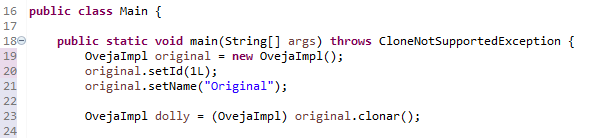
\includegraphics{images/creational/prototipe/prorotypeExample4.png}
\end{figure}

Como se puede observar, el patrón cumplió con su propósito creando una copia exacta de la oveja original

\begin{figure}[H]
	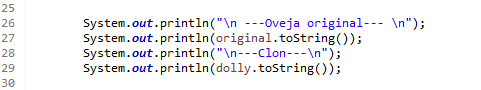
\includegraphics{images/creational/prototipe/prorotypeExample5.png}
\end{figure}

\begin{figure}[H]
	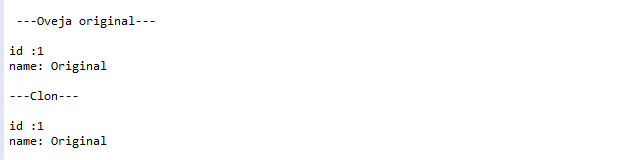
\includegraphics{images/creational/prototipe/prorotypeExample6.png}
\end{figure}

Sin embargo, a pesar que las ovejas tienen la misma información  no son el mismo objeto, por lo cual modificar la copia no afectará a la oveja original.

\begin{figure}[H]
	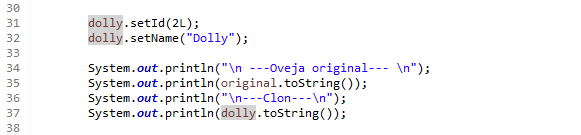
\includegraphics{images/creational/prototipe/prorotypeExample7.png}
\end{figure}

\begin{figure}[H]
	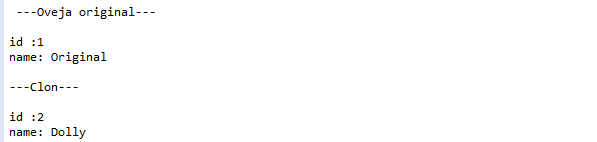
\includegraphics{images/creational/prototipe/prorotypeExample8.png}
\end{figure}

Debido a que las ovejas no son iguales, se puede concluir que hacen referencia a objetos diferentes en la aplicación.

\begin{figure}[H]
	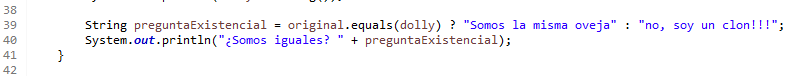
\includegraphics{images/creational/prototipe/prorotypeExample9.png}
\end{figure}

\begin{figure}[H]
	
\includegraphics{images/creational/prototipe/prorotypeExample10.png}
\end{figure}
\subsection{Builder}

\textbf{Definición:} El patron builder o constructor tiene el objetivo de permitir la creación de objetos complejos mediante un intermediario mas simple que encapsule la lógica asociada a la creación del objeto requerido.

\textbf{Motivación:} Por lo general, los lenguajes orientados a objetos permiten la creación de nuevas instancias de un objeto a través del uso de constructores y facilitan la definición de sus propiedades mediante el uso de su setter. Sin embargo, en algunas ocasiones un objeto puede tener múltiples combinaciones de sus propiedades o necesita ser inmutable, para estos casos la solución mas común es crear constructores específicos para cada combinación o mediante funciones que se encarguen de fijar sus atributos. Esto no es incorrecto y corresponde al diseño orientado a objetos, pero trae como desventaja que con el tiempo el código resultante sea demasiado extenso dificultando su mantenimiento.

\textbf{¿Como puedo implementar un builder?:} El patrón define una clase Builder cuyo objetivo es encapsular toda la lógica necesaria para crear el objeto. Particularmente, JAVA utiliza un builder muy conocido y utilizado por los desarrolladores (la clase StringBuilder) que encapsula toda la lógica involucrada en la creación de Strings complejos.

\textbf{Escenarios de aplicación:}

\begin{itemize}
	\item Existen muchas configuraciones posibles para la creación de un objeto.
	\item Se desea prescindir de multiples constructures en la implementación.
	\item La creación de un objeto complejo debe ser independiente de las partes que lo componen y debe ser lo suficientemente genérica para soportar múltiples representaciones del objeto.
	\item Crear una estructura genérica para facilitar los test de una clase.
	\item El objeto que se va a construir es inmutable
\end{itemize}

\textbf{Modelo UML:}

El patrón se centra en la definición de una clase Builder encargada de crear la estructura del objeto que se pretende construir. El truco fundamental para la abstracción del builder es la definición de métodos públicos que asocien cada propiedad al objeto y retornen la instancia del builder, lo cual permite que el objeto sea construido de manera dinámica de acuerdo a la necesidad del usuario. Finalmente, el builder cuenta con un método \textbf{build()} que se retorna la instancia del nuevo objeto al usuario.

\begin{figure}[H]
	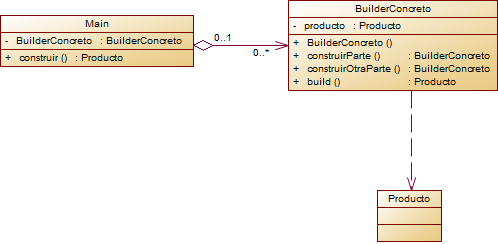
\includegraphics[width=0.9\textwidth]{images/creational/builder/builder.png}
\end{figure}

\textbf{Ejemplo conceptual:} En física, la teoría de cuerdas propone la existencia de múltiples Universos, cada uno con sus propias propiedades físicas inmutables.

Se solicita a un desarrollador crear un programa computacional que simule la creación de Universos de una manera sencilla y compacta. Para simplificar el problema, asumiremos que un Universo puede ser caracterizado en función de: un identificador, un código único, su masa, el porcentaje de materia barionica que posee (la materia barionica es la materia de la cual estamos compuestos), su porcentaje de materia oscura y su porcentaje de energía oscura (en física y en astronomía se da el indicativo de oscuro a todo aquello que no tenemos la mas remota idea de que pueda ser), y sus galaxias.

En general, cualquier objeto puede ser identificado a partir de un id y código únicos, por ello se crea una clase General que nos permita obtener estos atributos para cualquier clase en el dominio de la aplicación.

\begin{figure}[H]
	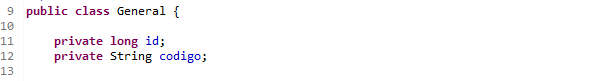
\includegraphics{images/creational/builder/builderExample1.png}
\end{figure}

Adicionalmente, se crea la estructura necesaria para crear nuevos Universos. Finalmente se extiende de la clase General para obtener los atributos comunes.

\begin{figure}[H]
	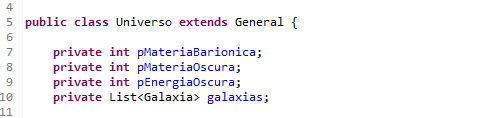
\includegraphics{images/creational/builder/builderExample2.png}
\end{figure}

De manera análoga, se crea la estructura necesaria para crear nuevas galaxias (cada galaxia podría tener a su vez estrellas que contengan planetas, pero eso no nos interesa por ahora).

\begin{figure}[H]
	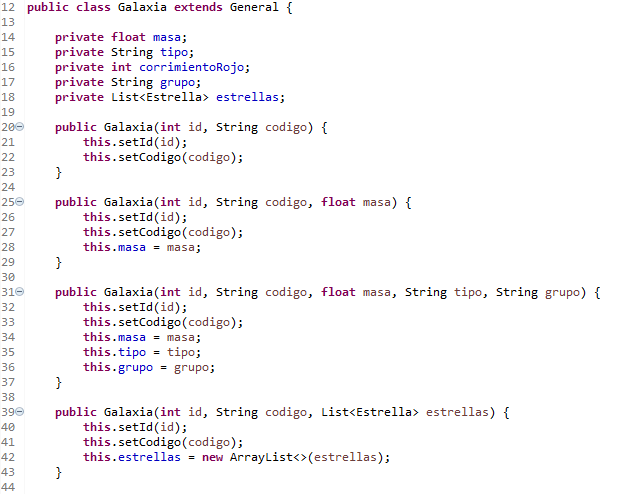
\includegraphics{images/creational/builder/builderExample3.png}
\end{figure}

 Como se puede observar, se decidió deliberadamente definir varios constructores en la clase Galaxia para ilustrar un punto. Sin la definición de un builder, cada vez que se quiera crear una nueva galaxia con características particulares sería necesario crear un nuevo constructor o fijar cada atributo uno a uno a través de sus metodos get. Esto es poco práctico y con el paso del tiempo la clase se comienza a hacer bastante extensa dificultando su mantenimiento. Por ahora nos enfocaremos en un builder para nuestro Universo, mas adelante buscaremos el mecanismo para crear nuevas galaxias de una manera mas adecuada.
 
 Por otro lado, se define una clase UniversoBuilder que a su vez contendrá el Universo en cuestión. Inicialmente, se crea la estructura básica con un constructor que inicialice los atributos obligatorios y los valores por defecto.
 
 \begin{figure}[H]
	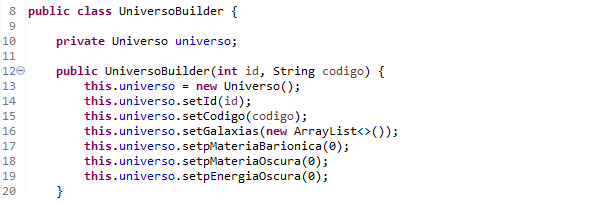
\includegraphics{images/creational/builder/builderExample4.png}
\end{figure}
 
 La clave para la implementación del patrón es la definición de métodos públicos que se encarguen de llenar el objeto y retornen el builder, esto permitirá la construcción del objeto de manera dinámica y garantizará que se pueda construir el objeto de acuerdo a las necesidades del usuario. Finalmente, se define un método build que retornará nuestro nuevo Universo.
 
 \begin{figure}[H]
	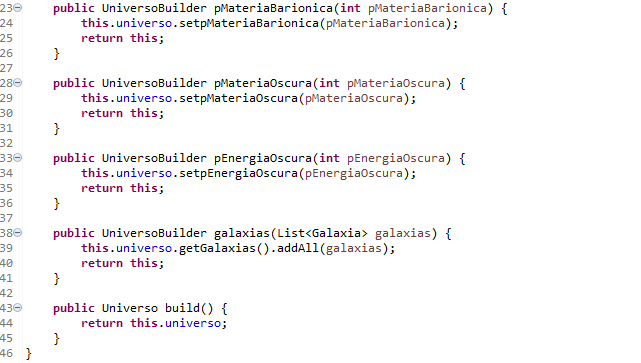
\includegraphics{images/creational/builder/builderExample5.png}
\end{figure}
 
 Gracias a esto, una clase externa ahora puede crear Universos de una manera compacta y de acuerdo a su necesidad.
 
 \begin{figure}[H]
	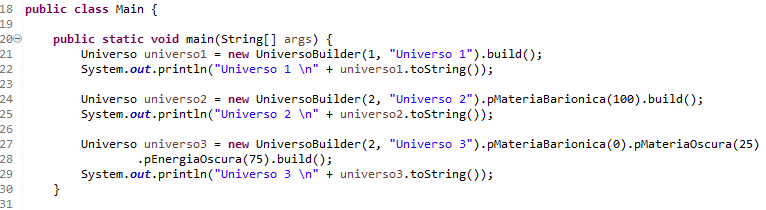
\includegraphics{images/creational/builder/builderExample6.png}
\end{figure}
 
 \begin{figure}[H]
	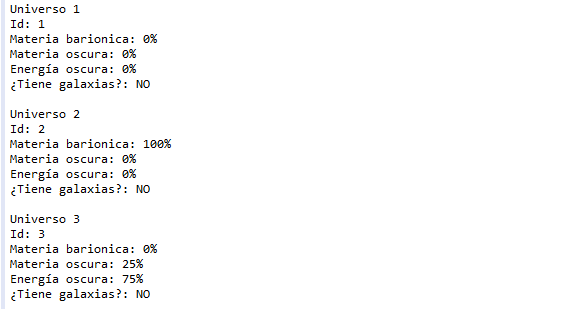
\includegraphics{images/creational/builder/builderExample7.png}
\end{figure}

Hasta ahora las cosas van bastante bien ¿pero que pasaría si necesitaramos crear nuevas galaxias? Supongamos que queremos crear un nuevo Universo con varias galaxias de diferentes características. De acuerdo a la definición actual se tendría que llamar un constructor diferente para cada configuración o crear el objeto y fijar sus atributos uno a uno, lo cual es poco práctico.

\begin{figure}[H]
	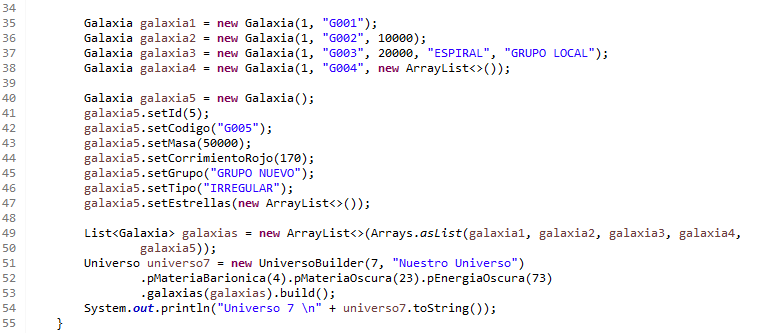
\includegraphics{images/creational/builder/builderExample8.png}
\end{figure}

Sin embargo, se puede definir una clase GalaxiaBuilder encargada de simplificar la creación de los objetos y prescindir de los constructores en el objeto original. Gracias a esto, la instanciación de nuevas Galaxias se haría desde el builder.

\begin{figure}[H]
	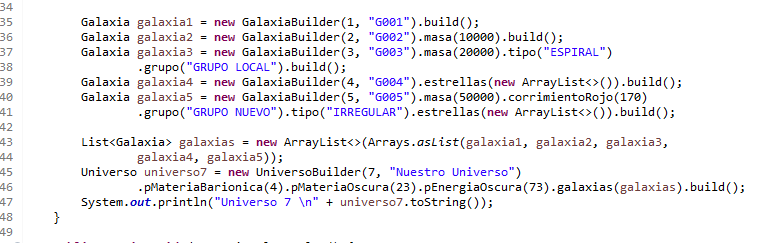
\includegraphics{images/creational/builder/builderExample9.png}
\end{figure}

Como resultado, el builder permite abstraer la construcción de cualquier combinación del objeto a una estructura mas compacta. Inicialmente podría pensarse que no hay una diferencia sustancial con respecto a la definición inicial, pero la ventaja del builder radica en eliminar la definición de multiples constructores y hacer el código mas fácil de comprender y mantener. Como resultado, la clase Galaxia ya no necesita constructores.

\begin{figure}[H]
	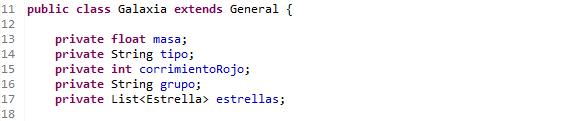
\includegraphics{images/creational/builder/builderExample12.png}
\end{figure}

Uno de los aspectos mas interesantes del patrón builder es que gracias a su flexibilidad puede implementarse de varias formas. A continuación, se presentará otra forma en la cual se podría resolver el problema presentado anteriormente. Para ello, se cambia la definición del builder a una clase estática contenida en el objeto que vamos a construir, en este caso nuestro Universo.

\begin{figure}[H]
	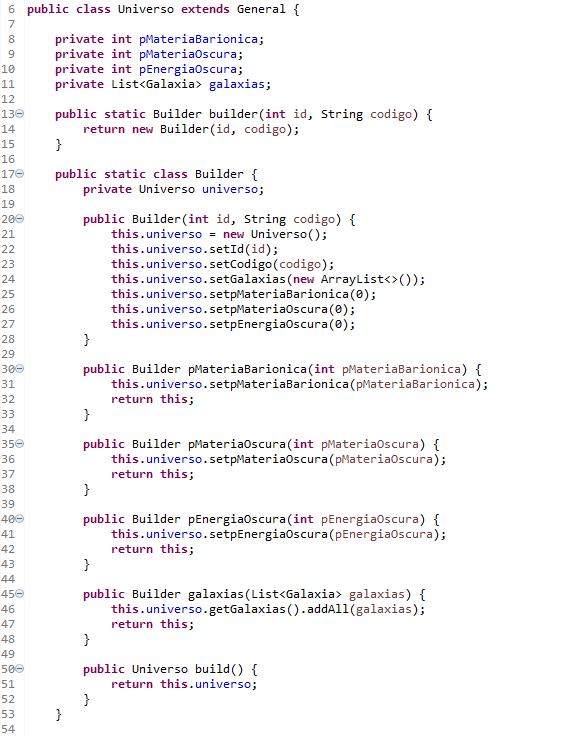
\includegraphics{images/creational/builder/builderExample13.png}
\end{figure}

De manera analoga, se crea la clase Galaxia con su propio builder. El aspecto mas importante que se debe considerar al utilizar esta aproximación es la definición de un constructor estático que permita la creación del builder contenido en la clase y que se va a encargar de construir el objeto.

\begin{figure}[H]
	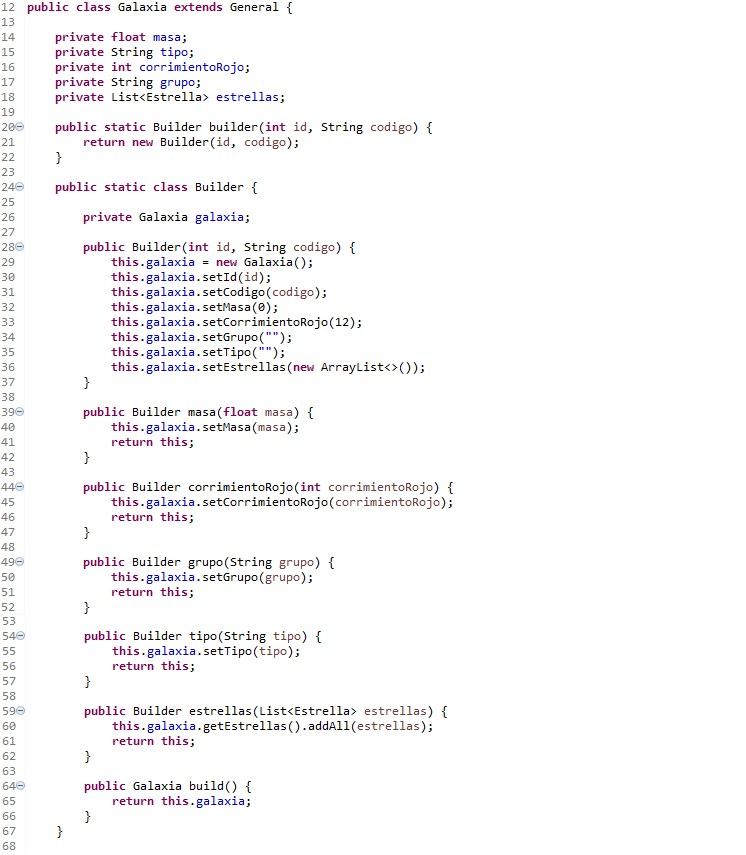
\includegraphics{images/creational/builder/builderExample14.png}
\end{figure}

Debido a que cada builder está acoplado al objeto que se va a crear es posible instanciar el objeto directamente desde la clase de manera estática.

\begin{figure}[H]
	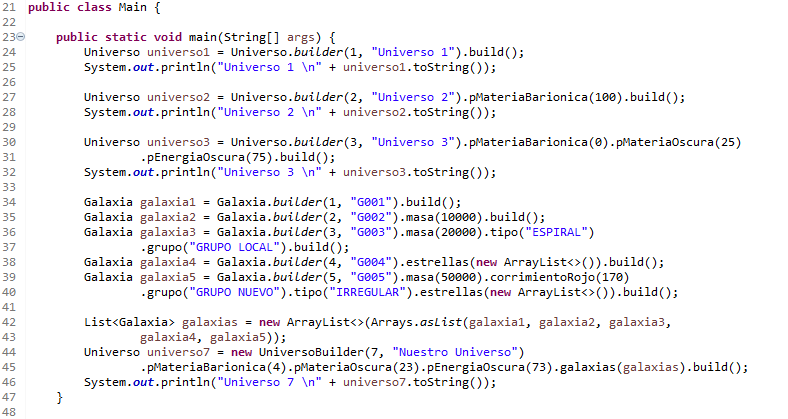
\includegraphics{images/creational/builder/builderExample15.png}
\end{figure}

Un aspecto interesante del patrón builder es su flexibilidad al permitir que su implementación sea realizada de diferentes maneras, en este libro se presentaron dos aproximaciones frecuentemente utilizadas en muchos frameworks. Sin embargo, otros autores como el Gof o Eric y Elizabeth Freeman presentan aproximaciones diferentes a esta, invito a cualquier lector curioso a indagar sobre las diferentes maneras de implementar el patrón builder. 

En este punto ya hemos logrado implementar el patrón builder y descubrimos que tiene grandes ventajas en la construcción de objetos complejos. Sin embargo, este patrón no debe ser utilizado a la ligera y el analisis de cuando debería usarse recae en la solución que se esté llevando a cabo. Se debe tener en cuenta que el patrón hace el código mas flexible con un costo (se requiere una clase adicional que aumenta el consumo de recursos en la aplicación). Es criterio del desarrollador decidir cuando el patrón builder es la mejor opción.
